\documentclass[a4paper,twoside,10pt,french,twocolumn]{scrartcl}
\usepackage[T1]{fontenc}
\usepackage{titlesec}
\usepackage{ulem}
\usepackage[dvipsnames]{xcolor}
\usepackage{color}
\usepackage{babel} 
\usepackage{pst-tree}
\usepackage{tikz}
\usetikzlibrary{trees}
\usepackage{helvet} 
\usepackage[utf8]{inputenc}
\usepackage[T1]{fontenc}
\usepackage{geometry}
\title{Chapitre 3 : Probabilités conditionnelles et évènements indépendants}
\date{}
 \renewcommand*\familydefault{\sfdefault} 
\geometry{a4paper}
% ------------------------------------------------------------------------
% ----------- Création des commandes de couleur pour les titres ----------
% ------------------------------------------------------------------------
\newcommand{\sectionred}[1]{{\color{red}{\uuline{\color{black}#1}}}}
\newcommand{\sectiongreen}[1]{{\color{ForestGreen}{\uuline{\color{black}#1}}}}
\newcommand{\sectionblue}[1]{{\color{NavyBlue}{\uuline{\color{black}#1}}}}
\begin{document}
\maketitle
% ------------------------------------------------------------------------
% ---------------- Modification des titres de niveau 1,2 et 3 ------------
% ------------------------------------------------------------------------
\titleformat
{\section} % command
%[display] % shape
{\Large} % format
{{\color{red}\uuline{\color{black}\thesection -}}} % label
{0ex} % sep
{\sectionred} % before-code
[] % after-code

\titleformat
{\subsection}%[display] % shape
{\Large} % format
{{\color{ForestGreen}\uuline{\color{black}\thesubsection -}}} % label
{0ex} % sep
{\sectiongreen} % before-code
[] % after-code

\titleformat
{\subsubsection} % command
%[display] % shape
{\large} % format
{{\color{NavyBlue}\uuline{\color{black}\thesubsubsection -}}} % label
{0ex} % sep
{\sectionblue} % before-code
[] % after-code

% --------------------------------------------------------------------------------
% ---------------- Début du corps du document ------------------------------------
% --------------------------------------------------------------------------------

\section{Rappels}
\subsection{Définitions}
\subsubsection{Expérience\:aléatoire}
Expérience dont on connait les issues, mais pas laquelle sortira.
\subsubsection{Univers}
Ensemble de toutes les issues possibles. Noté $\Omega$
\subsubsection{Inter/Ou}
La probabilité d'obtenir l'évènement A \uuline{et} B se note $P(A \cap B)$.
La probabilité d'obtenir l'évènement A \uuline{ou} B se note $P(A \cup B)$.
\subsection{Règle}
La somme de toutes les probabilités d'une expérience est égale à 1.
\section{Probabilité\:conditionnelle}
\subsection{Définition}
$P_A(B)$ est la probabilité que l'évènement $B$ se réalise sachant que l'évènement $A$ est déjà réalisé.
\subsection{Formules}
\[P_A(B) = \frac{P(A \cap B)}{P(A)} \: \texttt{ou} \: P_B(A) = \frac{P(A \cap B)}{P(B)}\]
\[P(A \cap B) = P(A) \times P_A(B) = P(B) \times P_B(A)\]
\section{Arbre\:pondéré}
\subsection{Définition}
C'est un arbre dans lequel on inscrit les probabilités de chaque évènements sur les branches.
\subsection{Règles}
\begin{itemize}
\item La somme des probabilités des branches issues d'un même noeud est 1. 
\item La probabilité de l'évènement indiqué au bout du chemin est égal aux produit des probabilités rencontrées sur les branches.
\end{itemize}
\subsection{Modèle}
\subsubsection{Général}
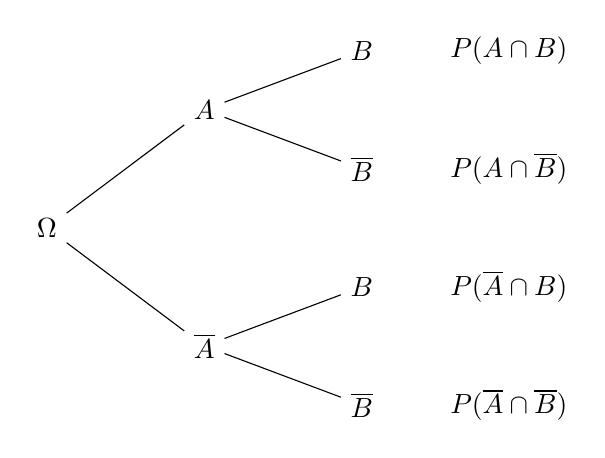
\begin{tikzpicture}
[level 1/.style={level distance=2cm,
sibling distance=3cm},
level 2/.style={level distance=2cm,
sibling distance=1.5cm}]
\node {$\Omega$} [grow'=right]
child {node {\textcolor{black}{$A$}}
child {node {\textcolor{black}{$B$}}
node[right=1cm] {$P(A\cap B)$}
edge from parent node[above] {}
}
child {node {\textcolor{black}{$\overline{B}$}}
node[right=1cm] {$P(A \cap \overline{B})$}
edge from parent node[below] {}
}
edge from parent node[above] {}
}
child {node {\textcolor{black}{$\overline{A}$}}
child {node {\textcolor{black}{$B$}}
node[right=1cm] {$P(\overline{A} \cap B)$}
edge from parent node[above] {}
}
child {node  {\textcolor{black}{$\overline{B}$}}
node[right=1cm] {$P(\overline{A} \cap \overline{B})$}
edge from parent node[below] {}
}
edge from parent node[below] {}
}
;
\end{tikzpicture}
\subsubsection{Exemple}
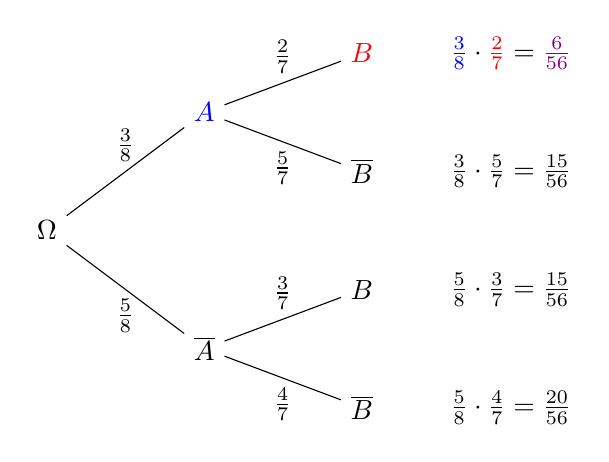
\begin{tikzpicture}
[level 1/.style={level distance=2cm,
sibling distance=3cm},
level 2/.style={level distance=2cm,
sibling distance=1.5cm}]
\node {$\Omega$} [grow'=right]
child {node {\color{Blue}{$A$}}
child {node {\color{Red}{$B$}}
node[right=1cm] {${\color{Blue}{\frac{3}{8}}}\cdot{\color{Red}{\frac{2}{7}}} = {\color{Purple}{\frac{6}{56}}}$}
edge from parent node[above] {$\frac{2}{7}$}
}
child {node {\textcolor{black}{$\overline{B}$}}
node[right=1cm] {$\frac{3}{8}\cdot\frac{5}{7} = \frac{15}{56}$}
edge from parent node[below] {$\frac{5}{7}$}
}
edge from parent node[above] {$\frac{3}{8}$}
}
child {node {\textcolor{black}{$\overline{A}$}}
child {node {\textcolor{black}{$B$}}
node[right=1cm] {$\frac{5}{8}\cdot\frac{3}{7} = \frac{15}{56}$}
edge from parent node[above] {$\frac{3}{7}$}
}
child {node {\textcolor{black}{$\overline{B}$}}
node[right=1cm] {$\frac{5}{8}\cdot\frac{4}{7} = \frac{20}{56}$}
edge from parent node[below] {$\frac{4}{7}$}
}
edge from parent node[below] {$\frac{5}{8}$}
}
;
\end{tikzpicture}
\uline{Remarques} :
\begin{itemize}
\item $\frac{3}{8}+\frac{5}{8} = \frac{8}{8} = 1$
\item $P({\color{Blue}{A}}\cap {\color{Red}{B}}) = {\color{Blue}{\frac{3}{8}}}\cdot{\color{Red}{\frac{2}{7}}} = {\color{Purple}{\frac{6}{56}}}$
\end{itemize}
\section{évènements\:indépendants}
A et B sont indépendants
\begin{itemize}
\item si $P_A(B) = P(B)$ (ou $P_B(A) = P(A)$) ou
\item si $P(A \cap B) = P(A) \times P(B)$
\end{itemize}
\section{Probabilités\:totales}
\subsection{Définitions}
Une partition de l'univers sont les parties de $\Omega$ qui sont
\begin{itemize}
\item disjointes deux à deux
\item et dont la réunion est $\Omega$
\end{itemize}

\subsection{Propriétés}
Si $A_1$, $A_2$, $A_3$, $A_n$ forment une partition de l'univers, B est un évènement tels que : $P(B) = P(B \cap A_1) + P(B \cap A_2) + P(B \cap A_3) + P(B \cap A_n)$
\subsection{Exemple}
On reprend l'arbre de 3.3.2.
\[ P(B) = P(A \cup B) + P(\overline{A} \cup B) = \frac{6}{56} + \frac{20}{56} = \frac{26}{56} \]
\end{document}
